

\tikzset{every picture/.style={line width=0.75pt}} %set default line width to 0.75pt        

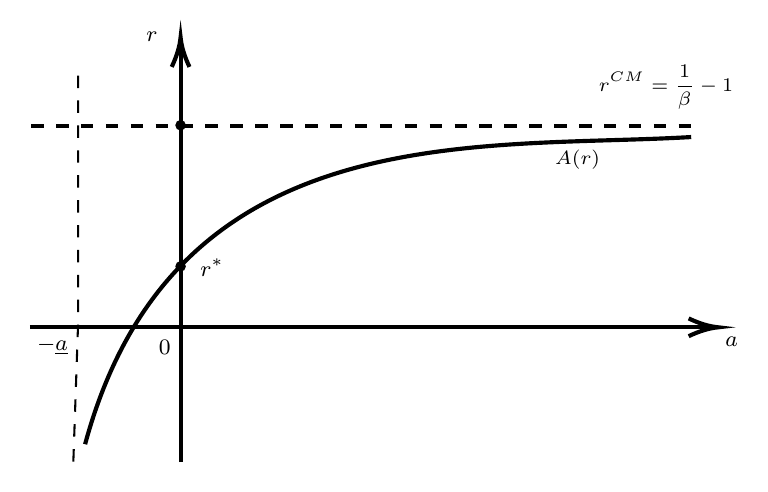
\begin{tikzpicture}[x=0.75pt,y=0.75pt,yscale=-1,xscale=1]
%uncomment if require: \path (0,326); %set diagram left start at 0, and has height of 326

%Straight Lines [id:da7110241033240954] 
\draw [line width=1.5]    (113.33,222) -- (442,222) ;
\draw [shift={(445,222)}, rotate = 180] [color={rgb, 255:red, 0; green, 0; blue, 0 }  ][line width=1.5]    (14.21,-4.28) .. controls (9.04,-1.82) and (4.3,-0.39) .. (0,0) .. controls (4.3,0.39) and (9.04,1.82) .. (14.21,4.28)   ;
%Straight Lines [id:da17023022650617547] 
\draw [line width=1.5]    (186,287) -- (186,85.33) ;
\draw [shift={(186,82.33)}, rotate = 90] [color={rgb, 255:red, 0; green, 0; blue, 0 }  ][line width=1.5]    (14.21,-4.28) .. controls (9.04,-1.82) and (4.3,-0.39) .. (0,0) .. controls (4.3,0.39) and (9.04,1.82) .. (14.21,4.28)   ;
%Curve Lines [id:da887933551738197] 
\draw [color={rgb, 255:red, 0; green, 0; blue, 0 }  ,draw opacity=1 ][line width=1.5]    (140,278.33) .. controls (183,119.33) and (330,136.33) .. (432,130.33) ;
%Straight Lines [id:da363676365000813] 
\draw [dash pattern={on 4.5pt off 4.5pt},color={rgb, 255:red, 0; green, 0; blue, 0 }  ,draw opacity=1 ][line width=1.5]    (114,125) -- (437,125) ;
%Straight Lines [id:da45020072866344707] 
\draw [line width=0.75]  [dash pattern={on 4.5pt off 4.5pt}]  (134.33,286.67) -- (136.67,218.67) -- (136.67,97.98) ;
%Straight Lines [id:da4086347964649337] 
\draw    (186,192.65) ;
\draw [shift={(186,192.65)}, rotate = 0] [color={rgb, 255:red, 0; green, 0; blue, 0 }  ][fill={rgb, 255:red, 0; green, 0; blue, 0 }  ][line width=0.75]      (0, 0) circle [x radius= 2.01, y radius= 2.01]   ;
%Straight Lines [id:da9545093660185393] 
\draw    (186,124.65) ;
\draw [shift={(186,124.65)}, rotate = 0] [color={rgb, 255:red, 0; green, 0; blue, 0 }  ][fill={rgb, 255:red, 0; green, 0; blue, 0 }  ][line width=0.75]      (0, 0) circle [x radius= 2.01, y radius= 2.01]   ;

% Text Node
\draw (365,135) node [anchor=north west][inner sep=0.75pt]  [font=\scriptsize,color={rgb, 255:red, 0; green, 0; blue, 0 }  ,opacity=1 ] [align=left] {$\displaystyle A( r)$};
% Text Node
\draw (168,78.14) node [anchor=north west][inner sep=0.75pt]  [font=\footnotesize] [align=left] {$\displaystyle r$};
% Text Node
\draw (386,94) node [anchor=north west][inner sep=0.75pt]  [font=\scriptsize,color={rgb, 255:red, 0; green, 0; blue, 0 }  ,opacity=1 ] [align=left] {$\displaystyle r^{CM} =\frac{1}{\beta } -1$};
% Text Node
\draw (115.33,225) node [anchor=north west][inner sep=0.75pt]  [font=\footnotesize] [align=left] {$\displaystyle -\underline{a}$};
% Text Node
\draw (174,226.66) node [anchor=north west][inner sep=0.75pt]  [font=\footnotesize] [align=left] {$\displaystyle 0$};
% Text Node
\draw (447,225) node [anchor=north west][inner sep=0.75pt]  [font=\footnotesize] [align=left] {$\displaystyle a$};
% Text Node
\draw (194,187.66) node [anchor=north west][inner sep=0.75pt]  [font=\footnotesize] [align=left] {$\displaystyle r^{*}$};


\end{tikzpicture}